\documentclass[tikz,dvisvgm]{standalone}

\usepackage{cmbright}
\usepackage{amsmath} % for aligned
\usepackage{listofitems} % for \readlist to create arrays
\usetikzlibrary{arrows.meta} % for arrow size
\usepackage[outline]{contour} % glow around text
\contourlength{1.4pt}

% COLORS
\usepackage{xcolor}
\colorlet{myred}{red!80!black}
\colorlet{myblue}{blue!80!black}
\colorlet{mygreen}{green!60!black}
\colorlet{myorange}{orange!70!red!60!black}
\colorlet{mydarkred}{red!30!black}
\colorlet{mydarkblue}{blue!40!black}
\colorlet{mydarkgreen}{green!30!black}

% STYLES
\tikzset{
  >=latex, % for default LaTeX arrow head
  node/.style={thick,circle,draw=myblue,minimum size=22,inner sep=0.5,outer sep=0.6},
  node in/.style={node,green!20!black,draw=mygreen!30!black,fill=mygreen!25},
  node hidden/.style={node,blue!20!black,draw=myblue!30!black,fill=myblue!20},
  node convol/.style={node,orange!20!black,draw=myorange!30!black,fill=myorange!20},
  node out/.style={node,red!20!black,draw=myred!30!black,fill=myred!20},
  connect/.style={thick,mydarkblue}, %,line cap=round
  connect arrow/.style={-{Latex[length=4,width=3.5]},thick,mydarkblue,shorten <=0.5,shorten >=1},
  node 1/.style={node in}, % node styles, numbered for easy mapping with \nstyle
  node 2/.style={node hidden},
  node 3/.style={node out}
}
\def\nstyle{int(\lay<\Nnodlen?min(2,\lay):3)} % map layer number onto 1, 2, or 3

\begin{document}

% DEEP CONVOLUTIONAL NEURAL NETWORK
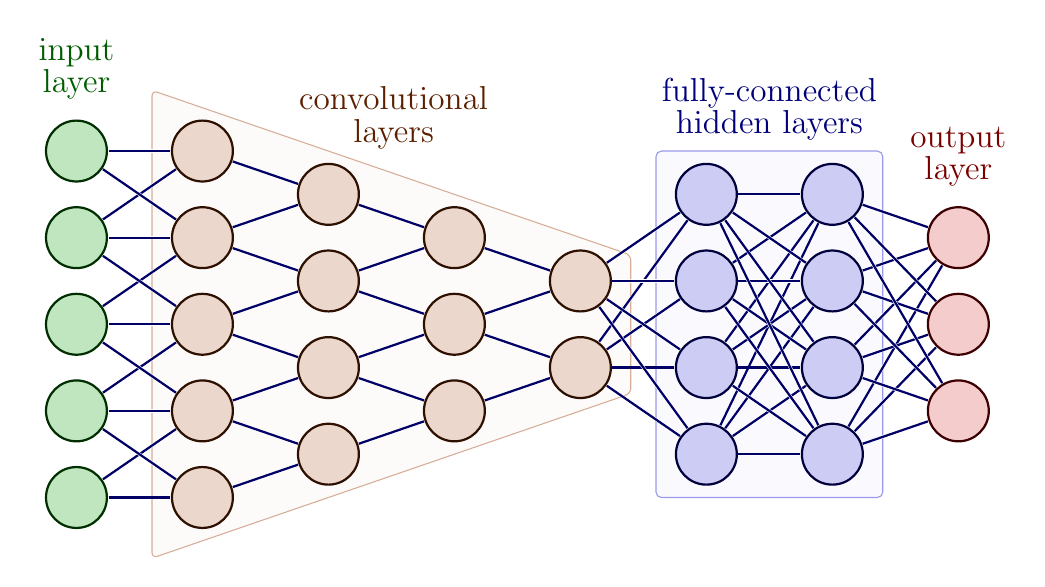
\begin{tikzpicture}[x=1.6cm,y=1.1cm]
  \large
  \message{^^JDeep convolution neural network}
  \readlist\Nnod{5,5,4,3,2,4,4,3} % array of number of nodes per layer
  \def\NC{6} % number of convolutional layers
  \def\nstyle{int(\lay<\Nnodlen?(\lay<\NC?min(2,\lay):3):4)} % map layer number on 1, 2, or 3
  \tikzset{ % node styles, numbered for easy mapping with \nstyle
    node 1/.style={node in},
    node 2/.style={node convol},
    node 3/.style={node hidden},
    node 4/.style={node out},
  }
  
  % TRAPEZIA
  \draw[myorange!40,fill=myorange,fill opacity=0.02,rounded corners=2]
    %(1.6,-2.5) rectangle (4.4,2.5);
    (1.6,-2.7) --++ (0,5.4) --++ (3.8,-1.9) --++ (0,-1.6) -- cycle;
  \draw[myblue!40,fill=myblue,fill opacity=0.02,rounded corners=2]
    (5.6,-2.0) rectangle++ (1.8,4.0);
  \node[right=19,above=3,align=center,myorange!60!black] at (3.1,1.8) {convolutional\\[-0.2em]layers};
  \node[above=3,align=center,myblue!60!black] at (6.5,1.9) {fully-connected\\[-0.2em]hidden layers};
  
  \message{^^J  Layer}
  \foreachitem \N \in \Nnod{ % loop over layers
    \def\lay{\Ncnt} % alias of index of current layer
    \pgfmathsetmacro\prev{int(\Ncnt-1)} % number of previous layer
    %\pgfmathsetmacro\Nprev{\Nnod[\prev]} % array of number of nodes in previous layer
    \message{\lay,}
    \foreach \i [evaluate={\y=\N/2-\i+0.5; \x=\lay; \n=\nstyle;}] in {1,...,\N}{ % loop over nodes
      %\message{^^J  Layer \lay, node \i}
      
      % NODES
      \node[node \n,outer sep=0.6] (N\lay-\i) at (\x,\y) {};
      
      % CONNECTIONS
      \ifnum\lay>1 % connect to previous layer
        \ifnum\lay<\NC % convolutional layers
          \foreach \j [evaluate={\jprev=int(\i-\j); \cconv=int(\Nnod[\prev]>\N); \ctwo=(\cconv&&\j>0);
                       \c=int((\jprev<1||\jprev>\Nnod[\prev]||\ctwo)?0:1);}]
                       in {-1,0,1}{
            \ifnum\c=1
              \ifnum\cconv=0
                \draw[connect,white,line width=1.2] (N\prev-\jprev) -- (N\lay-\i);
              \fi
              \draw[connect] (N\prev-\jprev) -- (N\lay-\i);
            \fi
          }
          
        \else % fully connected layers
          \foreach \j in {1,...,\Nnod[\prev]}{ % loop over nodes in previous layer
            \draw[connect,white,line width=1.2] (N\prev-\j) -- (N\lay-\i);
            \draw[connect] (N\prev-\j) -- (N\lay-\i);
          }
        \fi
      \fi % else: nothing to connect first layer
      
    }
  }
  
  % LABELS
  \node[above=3,align=center,mygreen!60!black] at (N1-1.90) {input\\[-0.2em]layer};
  \node[above=3,align=center,myred!60!black] at (N\Nnodlen-1.90) {output\\[-0.2em]layer};
  
\end{tikzpicture}


\end{document}